\section{Sequences and Series}

Notes from Oxford - M1 - Sequences and Series.

\subsection{Axioms for the real numbers}
\begin{mdframed}
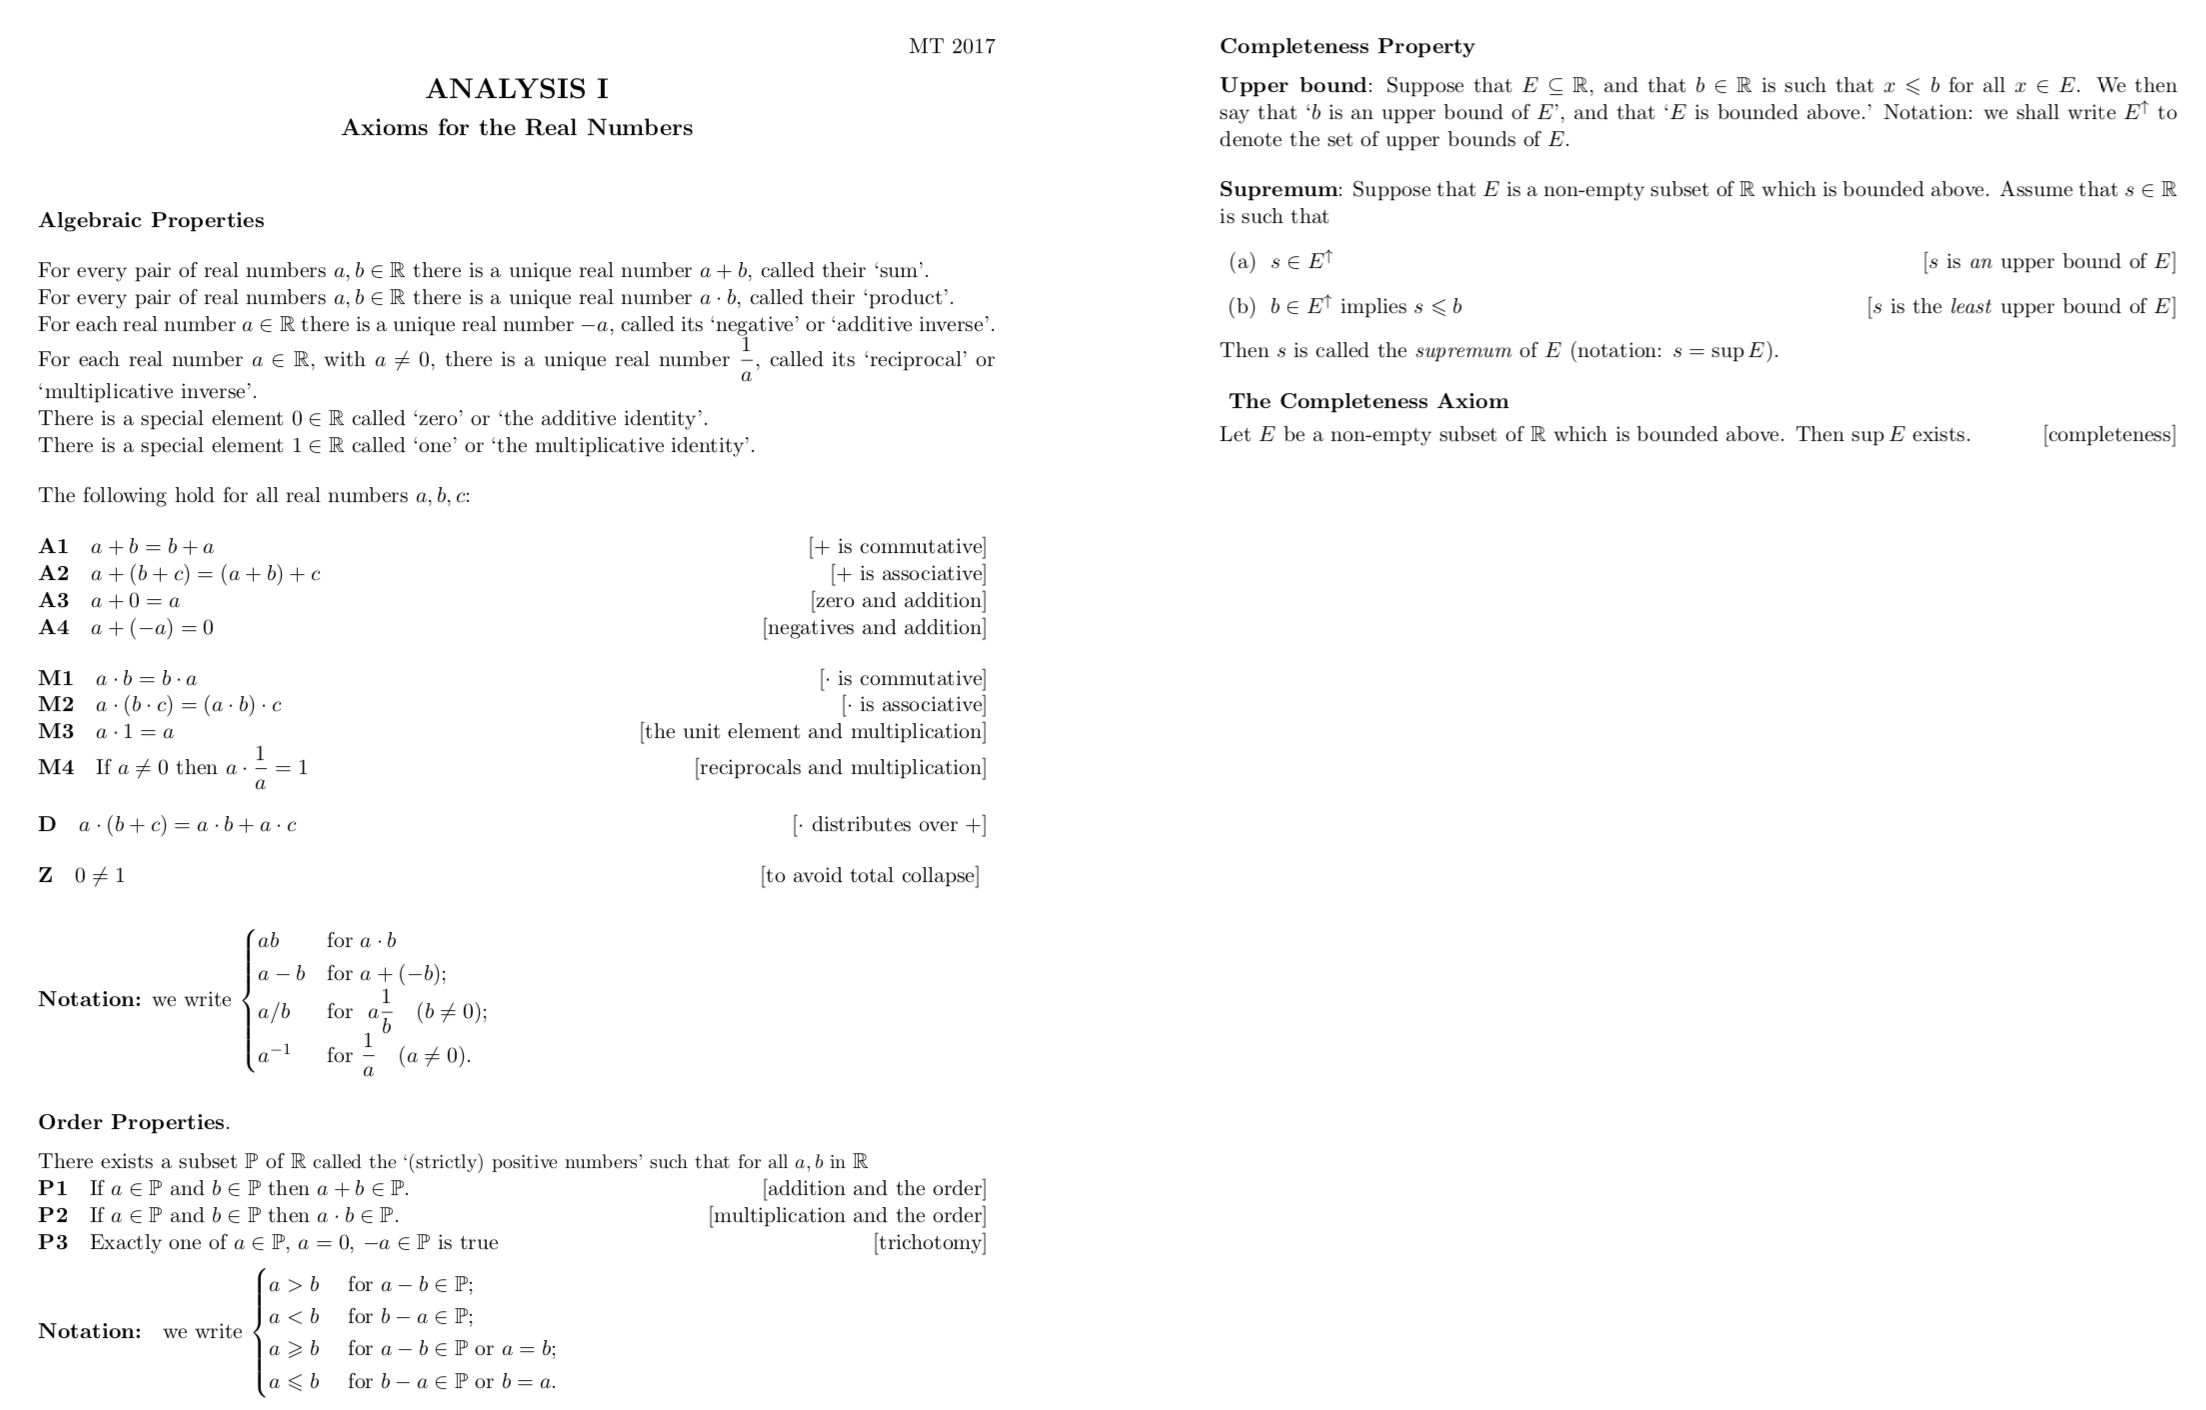
\includegraphics[width=400pt]{img/oxford-prelims-M2-analysis-I-axioms-for-real-numbers.png}
\end{mdframed}

\subsection{Approximation property of supremum}
\begin{theorem*}
  Let $S \subset \R$ be non-empty and bounded above (so $\sup S$ exists). For all $\delta > 0$,
  there exists $s_\delta \in S$ such that
  \begin{align*}
    \sup S - \delta < s_\delta \leq \sup S.
  \end{align*}
  \begin{intuition*}
    The supremum is either a member of $S$ or it is ``touching'' an element of $S$ with ``no gap''.
  \end{intuition*}
  \begin{proof}
    If $\sup S \in S$ then we can take $s_\delta = \sup S$ for all $\delta$ and we are done.

    So assume $\sup S \not\in S$. For a contradiction, suppose the negation of the claim, i.e. that
    there exists $\delta > 0$ such that for all $s \in S$ either $s \leq \sup S - \delta$ or
    $s > \sup S$. Since $s > \sup S$ is impossible by definition of $\sup$, we have that
    $s \leq \sup S - \delta$ for all $s \in S$. But then $\sup S - \delta$ is an upper bound for
    $S$ and $\sup S - \delta < \sup S$, a contradiction.
  \end{proof}
\end{theorem*}

\subsection{Archimedean Property of $\N$}
\begin{theorem*}\hspace{0pt}
  \begin{enumerate}
  \item $\N$ has no upper bound.
  \item For all $\epsilon > 0$ there exists $n \in \N$ such that $\frac{1}{n} < \epsilon$.
  \end{enumerate}
\end{theorem*}
\begin{proof}\hspace{0pt}
  \begin{enumerate}
  \item Suppose $\N$ has an upper bound. Then $\sup \N$ exists. By the Approximation Property
    there exists $n \in \N$ such that $\sup \N - \frac{1}{2} < n \leq \sup \N$. But then
    $n + 1 \in \N$ and $n + 1 > \sup N$, a contradiction. Therefore $\sup \N$ does not exist,
    therefore $\N$ has no upper bound.
  \item Since $\N$ has no upper bound, there exists $n \in \N$ such that $n > 1/\epsilon$,
    i.e. $1/n < \epsilon$.
  \end{enumerate}
\end{proof}

\subsection{Well-ordered property of $\N$}
\begin{theorem*}\hspace{0pt}
  Every nonempty subset of $\N$ has a minimum.
\end{theorem*}

\begin{proof}
  Let $\emptyset \neq S \subseteq \N \subset \R$. Note that $S$ is bounded below by 0, therefore
  $\inf S$ exists. Suppose $\inf S \not\in S$. By the Approximation Property, there exists
  $n_1 \in S$ such that $\inf S \leq n_1 < \inf S + 1$.

  We claim that $\inf S = n_1$. Suppose for a contradiction that $\inf S \neq n_1$. Then
  $n_1 = \inf S + \delta$ for some $0 < \delta < 1$. By the Approximation property again, there
  exists $n_2 \in S$ such that $\inf S \leq n_2 < n_1 < \inf S + 1$.

  But since $n_1 > n_2$ we have $n_1 \geq n_2 + 1$, therefore $n_1 \geq \inf S + 1$ which
  contradicts $n_1 < \inf S + 1$. Therefore $\inf S = n_1 \in S$ and $\min S$ exists.
\end{proof}

\begin{remark*}
  Similarly:
  \begin{enumerate}
    \item Every nonempty subset of $\Z$ that is bounded below has a minimum.
    \item Every nonempty subset of $\Z$ that is bounded above has a maximum.
  \end{enumerate}
\end{remark*}

\begin{intuition*}
  Because of the ``gappiness'' of $\N$ and $\Z$, bounded subsets must contain their suprema/infima.
\end{intuition*}

\subsection{Existence of ceil and floor}
\begin{definition*}[floor and ceil]
  Let $x \in \R$. Then floor of $x$ is $\floor{x} = \max\{n \in \Z ~|~ n \leq x\}$ and ceil of $x$
  is $\ceil{x} = \min\{n \in \Z ~|~ n \geq x\}$.
\end{definition*}

\begin{theorem*}[$\floor{x}$ and $\ceil{x}$ exist]~\\
  Let $x \in \R$. Define $S = \{n \in \Z ~|~ n \geq x\} \subset \R$. Note that $S$ is bounded below
  by $x$. Also $S$ is non-empty by the Archimedean Property of $\N$, since otherwise $x$ would be
  an upper bound for $\N$. Therefore $\ceil{x} = \min S$ exists by Well-Ordering.

  Similarly, $\floor{x}$ exists.
\end{theorem*}

\subsection{Existence of $\sqrt 2$}
\begin{theorem*}\label{existence-of-root-2}
  There exists a unique $a \in \R$ such that $a^2 = 2$.
\end{theorem*}

\begin{remark*}
  The only thing that ties the proof to the reals is that it relies on completeness ($\sup$
  exists). We know that $\sqrt 2 \not\in \Q$, therefore $\Q$ is not complete.
\end{remark*}

\begin{proof}
  Let $S = \{s \in \R ~|~ s^2 < 2\}$. Since $S$ is bounded above, $a := \sup S$ exists. We show
  that $a^2 = 2$ by showing that $a^2 < 2$ and $a^2 > 2$ lead to contradictions.

  Note that $1 \in S$, therefore $a \geq 1$.

  \begin{enumerate}
  \item {\bf Suppose $a^2 < 2$}. We seek an $h > 0$ such that $(a + h)^2 < 2$ since this would
    contradict the definition $a := \sup S$. Note that
    \begin{align*}
      (a + h)^2 - 2 &= a^2 + 2ah + h^2 - 2\\
                    &< a^2 - 2 + 3ah ~~~~~~~\text{if $h < a$}\\
                    &< 0             ~~~~~~~~~~~~~~~~~~~~~~\text{if $h < (2 - a^2)/3a$}.
    \end{align*}
    Therefore if we take $h < \min\(a, \frac{2 - a^2}{3a}\)$ then $a + h \in S$ which contradicts
    the definition $a := \sup S$.
  \item {\bf Suppose $a^2 > 2$}. By the Approximation Property for all $0 < h < 1$ we can find
    $s \in S$ such that $a - h < s$.  Therefore $(a - h)^2 < s^2 < 2$. We seek a value of $h$ such
    that $(a - h)^2 \geq 2$, which would be a contradiction. Note that $a^2 - 2ah < (a - h)^2$. If
    we take $h = (a^2 - 2)/2a$ then we have $a^2 - 2ah = 2 < (a - h)^2 < 2$, the desired
    contradiction.
  \end{enumerate}

  Finally to show that $a$ is unique, suppose that there exists $b \in \R$ with $b^2 = 2$. Then
  $0 = a^2 - b^2 = (a + b)(a - b)$ therefore $a = b$.
\end{proof}

\subsection{Connection between sequences and functions}

\begin{theorem*}
  The following two statements are equivalent:
  \begin{enumerate}
  \item $\lim_{x \to a} f(x) = L$
  \item For every sequence $(x_n)$ such that $x_n \neq a$
    \begin{align*}
      \(\lim_{n \to \infty} x_n = a\) \implies \(\lim_{n \to \infty} f(x_n) = f(a)\)
    \end{align*}
  \end{enumerate}
\end{theorem*}

\begin{intuition*}
  In other words:

  $\lim_{x \to a} f(x) = L$ if and only if the following is true:

  If $x_n \to a$ and $x_n \neq a$ then $f(x_n) \to f(a)$. I.e. $f$ is continuous.
\end{intuition*}

\begin{proof}

\end{proof}

\subsection{Limit of product is product of limits}
\red{TODO:check these proofs}
\begin{theorem*}\label{limit-of-product}~\\
  Let $\limxa f(x) = L_f$ and $\limxa g(x) = L_g$. Then
  $\limxa f(x)g(x) = L_fL_g$.
\end{theorem*}

\begin{proof}
  Note that
  \begin{align*}
    \limxa f(x)g(x) &= \limxa \Big((f(x) - L_f)(g(x) - L_g) + L_fg(x) + L_gf(x) - L_fL_g\Big)\\
                    &= L_fL_g + \limxa (f(x) - L_f)(g(x) - L_g),
  \end{align*}
  so we need to show that $\limxa (f(x) - L_f)(g(x) - L_g) = 0$. Fix $\epsilon > 0$. Since
  $\limxa (f(x) - L_f) = \limxa (g(x) - L_g) = 0$, there exists $\delta$ (pick the minimum of the
  two $\delta$s) such that whenever $|x - a| < \delta$
  \begin{align*}
    |(f(x) - L_f)| < \sqrt \epsilon ~~~\text{and}~~~|(g(x) - L_g)| < \sqrt \epsilon,
  \end{align*}
  therefore $|(f(x) - L_f)(g(x) - L_g) - 0| < \epsilon$ as required.
\end{proof}

\subsection{Limit of quotient is quotient of limits}
\red{TODO:check these proofs}
\begin{theorem*}~\\
  Let $\limxa f(x) = L_f$ and $\limxa g(x) = L_g \neq 0$. Then
  \begin{align*}
    \limxa \frac{f(x)}{g(x)} = \frac{L_f}{L_g}.
  \end{align*}
\end{theorem*}

\begin{proof}
  \red{TODO}
  \begin{align*}
    \limxa \frac{f(x)}{g(x)} - \frac{L}{M}
    = \limxa \frac{f(x)}{g(x)} - \frac{1}{g(x)} + \frac{1}{g(x)} - \frac{L}{M}
  \end{align*}

  Let $L_f = \limxa f(x)$ and $L_g = \limxa g(x) \neq 0$.

  Fix $\epsilon > 0$ and let $\delta_f$ and $\delta_g$ be such that
  \begin{align*}
    |x - a| < \delta_f \implies |f(x) - L_f| < \epsilon\\
    |x - a| < \delta_g \implies |g(x) - L_g| < \epsilon.
  \end{align*}
  Let $\delta = \min(\delta_f, \delta_g)$. Then
  \begin{align*}
    \frac{|f(x) - L_f|}{|g(x) - L_f|}
  \end{align*}
\end{proof}

\subsection{Exponential versus polynomial}
\begin{theorem*}
  $\frac{n^k}{c^n} \to 0$ as $n \to \infty$ for $k > 1$, $c > 1$.
\end{theorem*}
\begin{proof}
  Let $c = 1 + b$. Then
  \begin{align*}
    0
    < \frac{n^k}{c^n}
    &= \frac{n^k}{(1 + b)^n}\\
    &= \frac{n^k}{\sum_{i=1}^n\frac{n(n-1)\cdots(n-i+1)}{i!}b^i}\\
    &< \frac{n^k}{n(n-1)\cdots(n-k)}\frac{(k+1)!}{b^{k+1}} ~~~~~~~~\text{by retaining only the $i = k+1$ term, assuming $k+1 < n$}\\
    &< \frac{n^k}{n^{k+1}}\frac{(k+1)!}{b^{k+1}}\\
    &\to 0.
  \end{align*}
\end{proof}

\subsection{$O$ and $o$ notation}
\begin{definition*}~\\
  We write $a_n = O(b_n)$ if there exists $N \in \N$ and a constant $c > 0$ such that for all
  $n \geq N$
  \begin{align*}
    |a_n| \leq c|b_n|.
  \end{align*}
  We write $a_n = o(b_n)$ if $a_n/b_n$ is defined and $a_n/b_n \to 0$ as
  $n \to \infty$.
\end{definition*}

\begin{claim*}
  Let $a_k = \frac{(2k+1)(3k-1)}{(k+1)(k+2)^2}$. Then $a_k = O(k^{-1})$.
\end{claim*}

\begin{proof}
  \begin{align*}
    a_n &= \frac{(2n+1)(3n-1)}{(n+1)(n+2)^2}
         = \frac{6n^2 + n - 1}{n^3 + 5n^2 + 8n + 4}\\
        &=
          \frac{6}{n + 5 + 8n^{-1} + 4n^{-2}} +
          \frac{1}{n^2 + 5n + 8 + 4n^{-1}} -
          \frac{1}{n^3 + 5n^2 + 8n + 4}
  \end{align*}
\end{proof}


\subsection{Series}
\begin{definition*}~\\

   The following definition of ``series'' is non-standard and only half serious. In
  particular, note that by ``the 5-th term of a series'' one usually means $a_5$, not $s_5$. The
  word ``series'' tends to be used in a way that makes a formal definition difficult or impossible:


  Let $(a_n)$ be a real or complex sequence.

  $s_n := \sum_{k=1}^na_k$ is the $n$th {\bf partial sum}.

  The formal summation $\sum a_n := \sum_{n=1}^\infty a_n$ is the {\bf series}.

  {\bf Note}: The word ``series'' is not always clearly defined. Roughly speaking, a series is a
  ``summation of a sequence''; the limit in question may or may not exist.

  The series $\sum a_n$ converges iff $\lim_{n \to \infty} s_n$ exists.
\end{definition*}

\begin{intuition*}~\\
  The sequence $(a_n)$ is the sequence of ``steps''.

  The partial sum sequence $(s_n)$ is the sequence of locations visited.

  The series $\sum a_n$ converges if the sequence of locations converges.
\end{intuition*}

\subsection{Examples of series and power series}

\begin{tabular}{l|l|l}
  $n$th term             & Behaviour                                   & Name          \\[5pt]
  \hline&&\\
  $x^n$                  & Converges to $\frac{1}{1 - x}$ on $(-1, 1)$ & Geometric Series\\[5pt]
  $\frac{1}{n}$          & Diverges                                    & Harmonic Series \\[5pt]
  $\frac{1}{n\log n}$    & Diverges                                    &                 \\[5pt]
  $(-1)^{n+1}\frac{1}{n}$ & Converges to $\log 2$              & Alternating Harmonic Series \\[5pt]
  $\frac{x^n}{n}$        & Converges on $[-1, 1)$                      & Harmonic Series at $x=1$, Alternating Harmonic Series at $x=-1$\\[5pt]
\end{tabular}

\subsection{Series convergence theorems}
\begin{theorem*}\hspace{0pt}
  \begin{enumerate}[label=(\roman*)]
  \item $a_n = s_n - s_{n-1}$ for $n \geq 2$.
  \item If the series converges then $a_n \to 0$.
  \item If $a_k \geq 0$ then the series is monotonic increasing (and therefore converges iff it is bounded above).
  \item {\bf Comparison test; simple form}: If $0 \leq a_k \leq Cb_k$ then:
    \begin{itemize}
    \item $\sum b_k$ converges $\implies \sum a_k$ converges.
    \item Therefore also the contrapositive: $\sum a_k$ diverges $\implies \sum b_k$ diverges.
    \end{itemize}
  \item {\bf Comparison test; limit form}: If $a_k, b_k > 0$ for all $k$ and
    $\frac{a_k}{b_k} \to L$ then
    \begin{itemize}
    \item $\sum b_k$ converges $\iff \sum a_k$ converges.
    \end{itemize}
  \item {\bf Cauchy convergence criterion}: series converges iff sequence of partial sums is
    Cauchy. Note that $s_n - s_m = a_{m+1} + \ldots + a_n$.
  \item {\bf Absolute convergence}: if the $\sum |a_k|$ series converges then the series converges.
  \item $\frac{1}{p^n}$ series converges iff $p > 1$.
  \end{enumerate}
\end{theorem*}

\begin{remark*}
  $a_n \to 0$ does not imply that the series converges. Counterexample: the harmonic series
  $a_n = \frac{1}{n}$.
\end{remark*}

\begin{proof}\hspace{0pt}
  \begin{enumerate}[label=(\roman*)]
  \item Assume $s_n \to L$. We have $a_n = s_{n} - s_{n-1} \to L - L = 0$.
  \end{enumerate}
\end{proof}

\begin{lemma}\label{even-and-odd-subsequences-lemma}
  Let $(a_n)$ be such that $(a_{2n})$ and $(a_{2n + 1})$ both converge to $L \in \R$. Then
  $a_n \to L$.
\end{lemma}

\begin{proof}
  Fix $\epsilon > 0$. Let $N_1 \in \N$ be such that $|a_{2n} - L| < \epsilon$ for all $n \geq N_1$
  and let $N_2 \in \N$ be such that $|a_{2n + 1} - L| < \epsilon$ for all $n \geq N_2$.

  Let $N = 2\max(N_1, N_2)$. Then $|a_n - L| < \epsilon$ for all $n \geq N$, therefore $a_n \to L$.
\end{proof}

\subsection{The Harmonic Series diverges}

\begin{theorem*}
  Let $a_n = \frac{1}{n}$. Then $\sum a_n$ diverges.
\end{theorem*}

\begin{intuition*}
  In the 14th Century, Nicole d'Oresme argued that the harmonic series diverges by grouping the
  terms, after the first two, into groups of size $2, 4, 8, \ldots$.
  \begin{align*}
    \sum_{k=1}^\infty \frac{1}{k}
    &= 1 + \frac{1}{2} +
    \(\frac{1}{3} + \frac{1}{4}\) +
    \(\frac{1}{5} + \frac{1}{6} + \frac{1}{7} + \frac{1}{8}\) +
    \ldots\\
    &> 1 + \frac{1}{2} + \frac{1}{2} + \frac{1}{2} + \ldots.
  \end{align*}
  The following proof formalizes the argument.
\end{intuition*}

\begin{proof}
  Let $s_n = \sum_{k=1}^\infty a_k$. Consider
  \begin{align*}
    |s_{2^{n + 1}} - s_{2^n}|
    &= \frac{1}{2^n + 1} + \frac{1}{2^n + 2} + \ldots + \frac{1}{2^{n+1}}\\
    &\geq \frac{1}{2^{n+1}}2^n ~~~~~~~~~~~~~~\text{(smallest term) x (number of terms)}\\
    &= \frac{1}{2}.
  \end{align*}
  Therefore $(s_n)$ is not Cauchy, so $(s_n)$ diverges, i.e. $\sum a_n$ diverges.
\end{proof}

\begin{proof}
  An alternative proof uses the Integral Test. Note that $\int \frac{1}{x} \dx = \log x +
  C$. Therefore $\int_1^\infty \frac{1}{x} \dx$ does not exist (divergent). \red{incomplete}
\end{proof}


\subsection{The Alternating Series Test}
\begin{theorem}
  The series $\sum_{k\geq 1}(-1)^{k-1}a_k$ converges if
  \begin{enumerate}[label=(\roman*)]
  \item $a_k \geq 0$
  \item $a_{k+1} \leq a_k$
  \item $a_k \to 0$.
  \end{enumerate}
\end{theorem}

\begin{proof}
  \begin{intuition*}
    The steps alternate in direction and each one is smaller than the last in magnitude, so they
    always remain ``inside the previous steps''. The sequence of even-numbered locations form the
    ``lower edge'' -- a monotone increasing sequence bounded above by the first location. The proof
    demonstrates that the sequence of odd-numbered locations converges to the same location as the
    even-numbered, and therefore that the full sequence converges.
  \end{intuition*}

  Let $(s_n)$ be the sequence of partial sums. Consider the subsequence $(s_{2n})$, i.e. the
  sequence of partial sums $s_2, s_4, \ldots$. From (i) and (ii) we have
  \begin{align*}
    s_{2n}   &= a_1 - a_2 + a_3 - a_4 + \ldots + a_{2n - 1} - a_{2n}\\
             &= a_1 - (a_2 + a_3) - \ldots - (a_{2n - 2} + a_{2n - 1}) - a_{2n}\\
            &\leq a_1.
  \end{align*}
  Note that $s_{2(n+1)} - s_{2n} = a_{2n+1} - a_{2n + 2} \geq 0$, therefore $(s_{2n})$is monotone
  increasing. Also it is bounded above by $a_1$. Therefore it converges. Let $s_{2n} \to L \geq 0$.

  Note also that
  \begin{align*}
    s_{2n-1} &= s_{2n} + a_{2n} \leq a_1.
  \end{align*}
  But by (iii) we have $a_{2n} \to 0$, therefore $s_{2n-1} \to L$ also. Therefore $s_n \to L$ by lemma \ref{even-and-odd-subsequences-lemma}.
\end{proof}


\subsection{Integral Test}

\begin{intuition*}
  Basically, if $f$ is continuous and monotone decreasing for $x > N$, then
  \begin{align*}
    \int_N^\infty f(x) \dx \leq \sum_{n=N}^\infty f(n) \leq f(N) + \int_N^\infty f(x) \dx. ~~~~~~~\text{(see diagram below)}
  \end{align*}
\end{intuition*}

\begin{theorem*}[Integral Test Theorem]
  Let $f:[1,\infty] \to [0, \infty]$ be decreasing and non-negative. Define
  \begin{align*}
    s_n = \sum_{k=1}^nf(k) ~~~~~~~~~~~~~ I_n = \int_1^n f(x) \dx ~~~~~~~~~~~~~ \sigma_n = s_n - I_n.
  \end{align*}
  Then $\sigma_n \to \sigma$, where $0 \leq \sigma \leq f(1)$.
\end{theorem*}

\begin{corollary*}[Integral Test]
  $(s_n)$ converges if and only if $(I_n)$ converges.
\end{corollary*}

\begin{intuition*}\hspace{0pt}
  \begin{mdframed}
    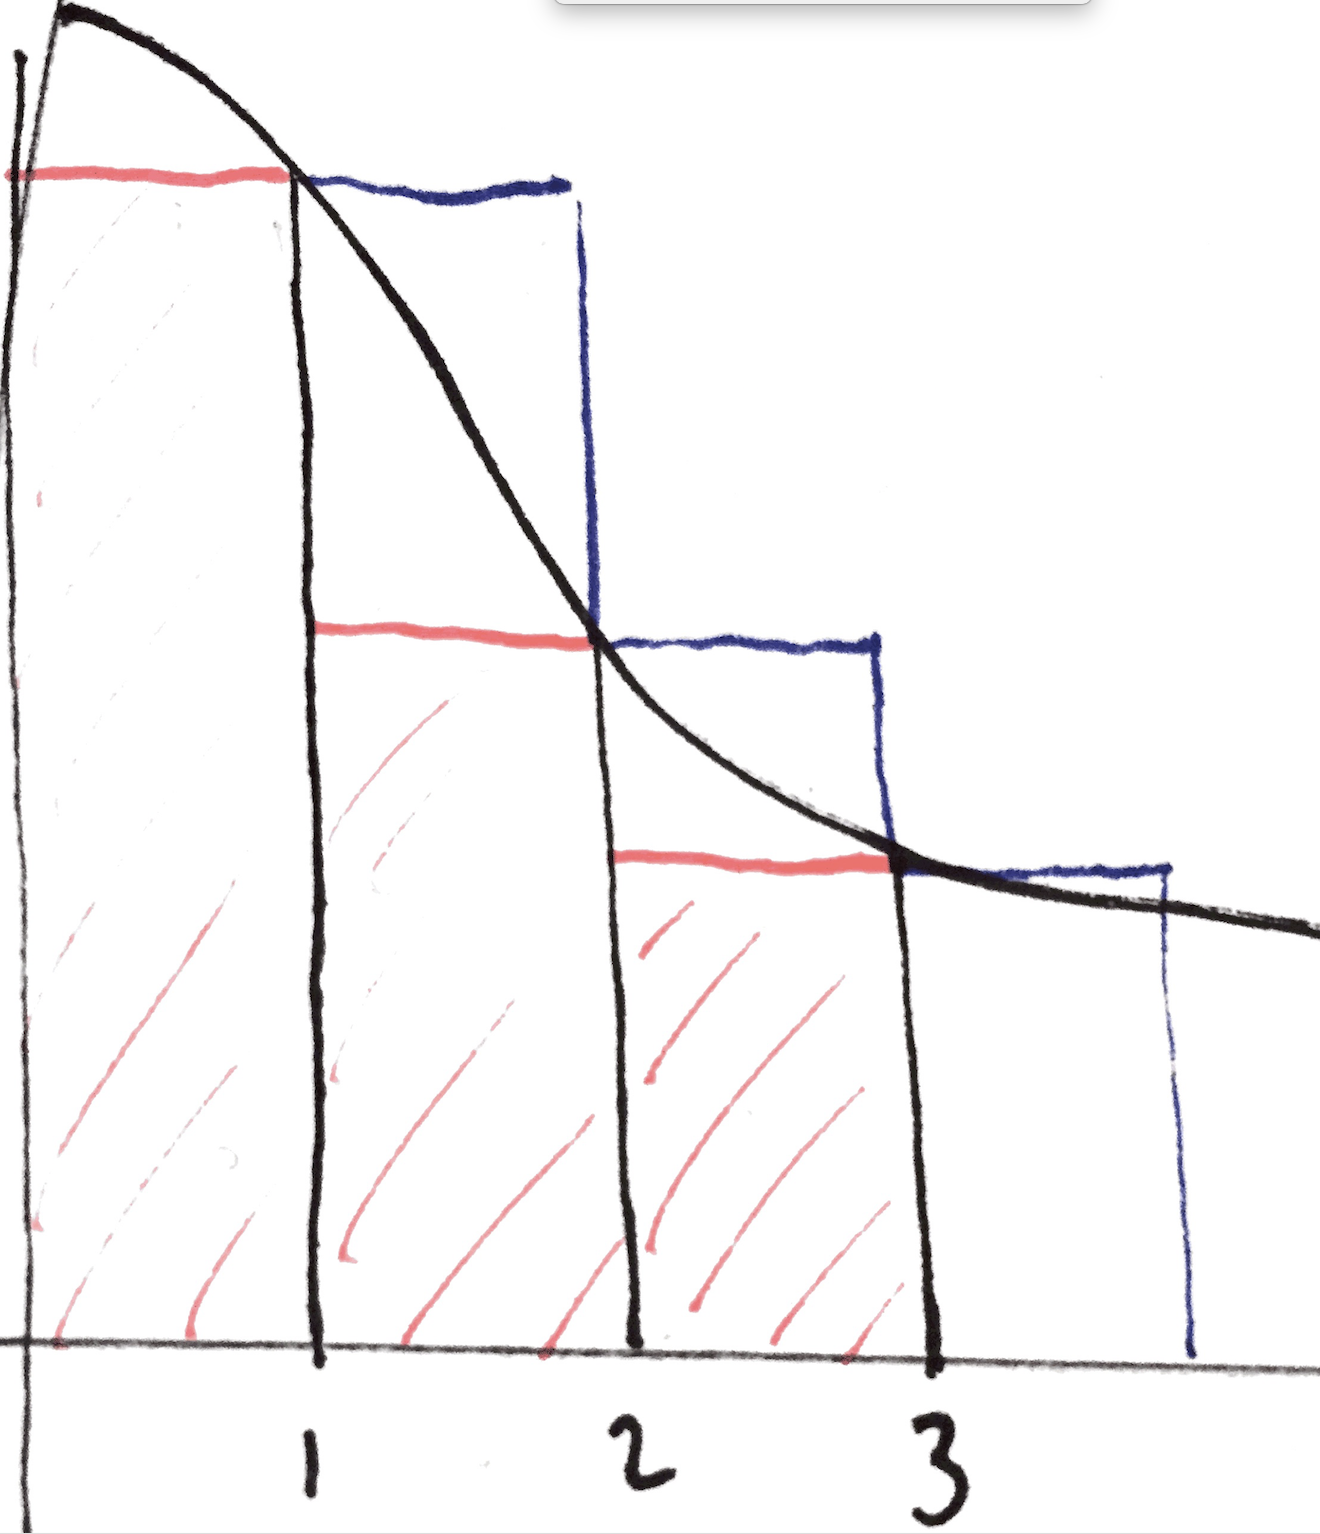
\includegraphics[width=200pt]{img/analysis--integral-test-theorem.png}

    The combined area of the 3 blue rectangles ($s_3 = f(1) + f(2) + f(3)$) exceeds the area
    $\int_1^3 f(x) \dx$. But the difference is less than $f(1)$. I.e.
    \begin{align*}
      f(1) + f(2) + f(3) \leq f(1) + \int_1^3 f(x) \dx
    \end{align*}


  \end{mdframed}
\end{intuition*}

\begin{proof}
  See notes.
\end{proof}



\subsection{Abel's theorem}
\begin{theorem*}
  Let $\sum_{n=0}^\infty a_nx^n$ be a power series with real coefficients $a_n$, convergent on
  $(-1, 1)$. Then $f$ given by $f(x) = \sum_{n=0}^\infty a_nx^n$ is left-continuous at $x=1$.
\end{theorem*}

\subsection{Alternating harmonic series}
\begin{theorem*}
  $\sum_{n=1}^\infty (-1)^{n+1}\frac{1}{n} = \log 2$.
\end{theorem*}

\begin{proof}

\end{proof}

Note that for $-1 < x < 1$ the series $\sum_{n=0}^\infty (-x)^n$ converges to
$\frac{1}{1+x}$. Therefore, using the term-by-term integration theorem for power series,
\begin{align*}
  \int\(\sum_{n=0}^\infty (-x)^n\) \dx
  = \sum_{n=0}^\infty \frac{(-x)^{n+1}}{n+1}
  = \sum_{n=1}^\infty \frac{(-x)^n}{n}
  = C + \log(1 + x),
\end{align*}
and taking $x=0$ shows that $C = 0$.

\begin{remark*}\hspace{0pt}
  \begin{enumerate}
  \item If it were valid to plug in $x=-1$ we would have the desired result
    $\sum_{n=1}^\infty \frac{(-1)^{n+1}}{n} = \log(2)$. However, this is not a proof, since the
    above argument is based on a geometric series with an interval of convergence of $-1 < x < 1$.
  \item The series $\sum_{n=1}^\infty \frac{(-1)^{n+1}}{n}$ does converge, by the Alternating
    Series Test. (The AST does not tell us what that limit is.)
  \end{enumerate}
\end{remark*}

Let $f$ be given by $f(x) = \sum_{n=1}^\infty \frac{(-x)^{n}}{n} = \log(1 + x)$. By Abel's theorem,
$f$ is continuous at the boundary point $x = 1$. I.e.
\begin{align*}
  \lim_{x\uparrow 1} \sum_{n=1}^\infty \frac{x^n}{n} = \log(2).
\end{align*}

\section{Continuity and Differentiability}
Notes from Oxford - M2 - Continuity and Differentiability.

\subsection{Limit point}
\begin{definition*}
Let $E \subset \R$. A point $p \in \R$ is a limit point of $E$ iff for all $\delta > 0$ there
exists $x \in E$ such that $0 < |x - p| < \delta$.
\end{definition*}
\begin{intuition*}
  A deleted ball, of arbitrarily small radius, placed over $p$, will capture at least one point of
  $E$.
\end{intuition*}

\subsection{Limit, Convergence}

\begin{definition*}[Limit of a sequence $(x_n)$]~\\
  $\lim_{n \to \infty} x_n = L$ iff for all $\epsilon > 0$ there exists $N \in \N$ such that
  $n > N \implies |x_n - L| < \epsilon$. The sequence is then said to \textit{converge} to $L$.
\end{definition*}

\begin{definition*}[Limit of a function $f:\R\to\R$]~\\
  $\lim_{x \to a} f(x) = L$ means: for all $\epsilon > 0$ there exists $\delta > 0$ such that
  $0 < |x - a| < \delta \implies |f(x) - L| < \epsilon$.
\end{definition*}

Equivalent notation: $f(x) \to L$ as $x \to a$

\begin{remark*}\hspace{0pt}
  \begin{enumerate}
  \item The value of $f$ at $a$ is irrelevant ($f$ need not be defined at $a$).
  \item $f$ must tend to $L$ from both sides.
  \end{enumerate}
\end{remark*}

\subsection{Limits involving $\infty$}

\begin{definition*}
  $\lim_{n \to \infty} x_n = \infty$ if for all $X \in \R$ there exists $N \in \N$ such that
  $n \geq N \implies x_n > X$.
\end{definition*}

\begin{definition*}
  $\lim_{x \to \infty} f(x) = L$ if for all $\epsilon > 0$ there exists $X \in \R$ such that
  $x > X \implies |f(x) - L| < \epsilon$.
\end{definition*}

\begin{theorem*}[I assume. Have not proved this.]
  $\lim_{x \to \infty} f(x) = L$ iff for all sequences $(x_n)$ such that
  $\lim_{n \to \infty}x_n = \infty$ we have $\lim_{n \to \infty} f(x_n) = L$.
\end{theorem*}

\subsection{Limits of functions - Examples}

\begin{example}
  Let $E = \R\setminus \{0\}$ and define $f:E \to \R$ by $f(x) = L$. Then 0 is a limit point of
  $E$ and $f(x) \to L$ as $x \to 0$.
\end{example}

\begin{proof}
  Fix $\delta > 0$. Then $\exists x ~ 0 < |x - 0| < \delta$ is true since we can choose
  $x = \frac{\delta}{2}$. Therefore 0 is a limit point of $E$.

  Fix $\epsilon > 0$. Let $\delta = 1$. Then
  $0 < |x - 0| < \delta \implies |f(x) - L| = 0 < \epsilon$.
\end{proof}

\subsection{Continuity of a function $f$}

\begin{definition*}
$f$ is continuous at $a$ if $\lim_{x \to a} f(x) = f(a)$.
\end{definition*}

Therefore, using the definition of limit, $f$ is continuous at $a$ iff for all $\epsilon > 0$
there exists $\delta > 0$ such that $|x - a| < \delta \implies |f(x) - f(a)| < \epsilon$.

\subsection{Uniform convergence and uniform continuity}

\begin{definition*}[Uniform convergence]
A sequence of functions $\{f_n\}_{n\geq 0}$ has a limit $f$ iff for every point
$x$ in the input set the sequence $\{f_n(x)\}_{n\geq 0}$ has limit $f(x)$.

They \textit{converge uniformly} to $f$ iff the same $m$ works for all input
values.
\end{definition*}

\begin{definition*}[Uniform continuity]
A function $f$ is uniformly continuous iff the same $\delta$ works for all $x_0$.

A function $f$ is uniformly continuous iff for all $\epsilon$, no matter how
small, a $\delta$ exists such that for all $x_0 \in U$, if $x$ is within
$\delta$ of $x_0$ then $f(x)$ is within $\epsilon$ of $f(x_0)$.
\end{definition*}

\subsection{Intermediate value theorem}
\begin{theorem*}
  Let $a, b \in \R$ with $b > a$, and $f:[a,b] \to \R$ be continuous. Let $u$ lie strictly between
  $f(a)$ and $f(b)$. Then there exists $c \in (a, b)$ such that $f(c) = u$.
\end{theorem*}

\begin{proof}
  Define $S := \{x \in [a, b] ~|~ f(x) < u\}$. Since $a \in S$, $S$ is non-empty. By completeness
  of reals $c := \sup S$ exists. The theorem now follows from continuity of $f$ at $c$. (Fix
  $\epsilon > 0$ and consider points $a^* \in (c - \delta, c)$ and $a^{**} \in (c, c + \delta)$,
  noting whether they are in $S$ and the $\epsilon-\delta$ continuity criterion.)
\end{proof}


\subsection{Mean-value theorem}
\begin{theorem*}
  Let $a, b \in \R$ with $b > a$, and $f:[a,b] \to \R$ be continuous on $[a, b]$ and differentiable
  on $(a, b)$. Then there exists $x \in (a, b)$ such that $f'(x) = \frac{f(b) - f(a)}{(b - a)}$.
\end{theorem*}


\subsection{Differentiability implies continuity}
\begin{theorem*}
  Let $f:\R\to\R$ be differentiable. Then $f$ is continuous.
\end{theorem*}

\begin{proof}~\\
  Let $a \in \R$. The claim is that $\limxa f(x) - f(a) = 0$. Since $f$ is differentiable,
  \begin{align*}
    f'(a) &= \lim_{x \to a} \frac{f(x) - f(a)}{x - a}
  \end{align*}
  exists. Therefore by \eqref{limit-of-product}
  \begin{align*}
    \lim_{x \to a} f(x) - f(a) = \lim_{x \to a} (x - a)\frac{f(x) - f(a)}{x - a} = 0\cdot f'(a) = 0.
  \end{align*}
\end{proof}

\begin{remark*}
  Intuitively it seems that differentiability implies continuity because, for the derivative to
  exist, the numerator $f(x) - f(a)$ must get small as $x\to a$, as the denominator $x - a$ does.
\end{remark*}


\newpage
\section{Metric Spaces}

\subsection{Metric space}
\begin{definition}
  Let $X$ be a set. Suppose $d:X \times X \to \R$ satisfies positivity, symmetry and the triangle
  equality. Then $d$ is a metric and $(X, d)$ is a metric space.
\end{definition}

\subsection{Open ball}
\begin{definition}
  Let $(X, d)$ be a metric space, $x \in X$ and $\delta > 0$. Then
  $B(x, \delta) := \{x \in X ~|~ d(x, x) < \delta\}$ is an open ball of radius $\delta$ centred at
  $x$.
\end{definition}

\begin{remark*}
  Also closed ball, $\leq$. E.g. singleton set.
\end{remark*}

\subsection{Ball-based continuity criterion}
\begin{lemma}
  $f$ is continuous at $x$ if for all $\epsilon > 0$ there exists $\delta > 0$ such that
  $f\(B(x, \delta)\) \subseteq B(f(x), \epsilon))$.

  Equivalently, $B(x, \delta) \subseteq f^\1\(B(f(x), \epsilon)\)$.
\end{lemma}

\subsection{Neighbourhood}
\begin{definition}
  Let $(X, d)$ be a metric space. $N \subseteq X$ is a neighbourhood of $x \in X$ if there exists
  $\delta > 0$ such that $B(x, \delta) \subseteq N$.
\end{definition}

\begin{remark*}
  $N$ is a neighbourhood of $x$ if a ball can be placed at $x$ without poking outside $N$.
\end{remark*}

\begin{theorem*}[Neighbourhoods are open]
  Let $(X, d)$ be a metric space and let $N \subseteq X$ be a neighbourhood of $x \in X$. Then $N$
  is open.

  \red{I don't think they are under the definitions here.}
\end{theorem*}

\begin{proof}
  Let $N = \{x' \in X ~|~ d(x, x') \leq 1\}$. Then $N$ is a neighbourhood of $x$ since
  $B(x, 0.5) \subset N$. But $N$ is not open.
\end{proof}


% \begin{proof}
%   Let $N \subseteq X$ be a neighbourhood of $x \in X$ and let $n \in N$. We wish to show that there
%   exists $\delta$ such that $B(n, \delta) \subseteq N$.

%   Since $N$ is a neighbourhood of $x$ there exists $\epsilon$ such that
%   $B(x, \epsilon) \subseteq N$.

%   Suppose $n \in B$.
% \end{proof}

\subsection{Open and closed subsets of a metric space}
\begin{definition}
  Let $(X, d)$ be a metric space. Then $U \subseteq X$ is open if it is a neighbourhood of all of
  its elements.

  $V \seq X$ is closed iff its complement in $X$ is open.
\end{definition}

\subsection{Topology on a metric space}
\begin{definition}
  Let $(X, d)$ be a metric space. The collection $\mc T$ of all open sets in the metric space is
  called the topology of $X$.
\end{definition}

\begin{remark*}
  Note that the definitions so far have the following dependency:

  (open set) $\larrow$ (neighbourhood) $\larrow$ (ball) $\larrow$ (metric),

  so they apply to metric spaces only.
\end{remark*}

\subsection{Open set-based continuity criterion}
\begin{theorem}
  Let $X$ and $Y$ be metric spaces and let $f:X \to Y$. Then

  $f$ is continuous at $x$ iff for every neighbourhood $N \subseteq Y$ of $f(x)$, the preimage
  $f^\1(N)$ is a neighbourhood of $x \in X$.

  $f$ is continuous iff for every open set $U$ of $Y$, $f^\1(U)$ is an open set of $X$.
\end{theorem}

\begin{remark*}
  So we have defined continuity in terms of open sets (the topology). This means that the metric is
  only relevant insofar as it induces the topology; two metric spaces with the same topology have
  the same notion of continuity.
\end{remark*}

\begin{proof}~\\
  Let $f$ be continuous at $x \in X$, and let $N \seq Y$ be a neighbourhood of $f(x)$.

  Then by definition of neighbourhood there exists a ball at $f(x)$ that stays within $N$.

  By continuity of $f$ the preimage of that ball is a superset of a ball at $x$.

  So the preimage of the ball is a neighbourhood of $x$. Therefore the preimage of $N$ is also.

  Conversely, ... similar.

  Let $f$ be continuous on $X$. Now every open set $U$ of $Y$ contains a ball around some point $y$...
\end{proof}

\subsection{Topology on a set, topological space}
\begin{definition}
  A topology on a set $X$ is a collection $\mc T$ of subsets of $X$, which are called the open
  sets. They must satisfy
  \begin{enumerate}
  \item closed under arbitrary unions. In particular, $\emptyset$ is an open set of $X$.
  \item closed under finite intersections. In particular, $X$ is an open set of $X$.
  \end{enumerate}
  A topological space is a pair $(X, \mc T)$.
\end{definition}

\begin{remark*}
  Criteria for closed sets follow by applying de Morgan's laws (closure under finite unions and
  arbitrary intersections).

  $f:X\to Y$ closed iff $f^\1(V)$ is closed for all closed sets $V \seq Y$.
\end{remark*}

\subsection{Limit point}
\begin{definition}
  Let $(X, d)$ be a metric space and $Z \seq X$ be any subset.

  $x \in X$ is a limit point of $Z$ if for all $\delta > 0$ the deleted open ball
  $B(x, \delta)\setminus\{x\}$ has non-empty intersection with $Z$.

  If $z$ is not a limit point of $Z$, then it is an isolated point.

  The set of limit points of $Z$ is denoted $Z'$, and it is clear that
  $Z_1 \seq Z_2 \implies Z_1' \seq Z_2'$.
\end{definition}

\begin{intuition*}
  $x \notin Z$ is a limit point of $Z$ iff it ``touches'' $Z$.

  $z \in Z$ is a limit point of $Z$ if it ``lies in a contiguous region of $Z$''

  An isolated point of $Z$ is what it sounds like.
\end{intuition*}

\begin{example*}~\\
  Let $Z = (0, 1] \cup \{2\}$.

  Intuitively, 0 is a limit point of $Z$ because it ``touches'' $Z$.

  Formally, 0 is a limit point of $Z$ because for all $\delta > 0$ the deleted open ball
  $B(0, \delta)$ contains a point $z > 0 \in Z$.

  Intuitively, 2 is an isolated point.

  Formally, 2 is not a limit point because $\(B(2, 0.5)\setminus\{2\}\) \cap Z = \emptyset$. And
  yet $2 \in Z$, therefore 2 is an isolated point.
\end{example*}

\subsection{Open sets theorems}
\begin{enumerate}
\item An open ball is open
\end{enumerate}

\subsection{Closed sets theorems}
\begin{enumerate}
\item A closed ball is closed
\end{enumerate}


\subsection{Continuity theorems}
\begin{enumerate}
\item $f:X \to Y$ is continuous if for every open ball in $Y$ there is an open ball in $X$ that
  maps inside it.
\item $f:X \to Y$ is continuous if the preimage of $B(f(x), \epsilon)$ in $Y$ is a ball
  $B(x, \delta)$ in $X$.
\item $f:X \to Y$ is continuous if the preimage of the neighbourhood of $f(x)$ is a neighbourhood
  of $x$.
\item $f:X \to Y$ is continuous if the preimage of every open set in $Y$ is an open set in $X$.
\end{enumerate}


\subsection{Continuity of a linear map}
\begin{theorem}
  Let $f:V \to W$ be a linear map between normed vector spaces. Then $f$ is continuous if and only
  if $\{\norm{f(x)} : \norm{x} \leq 1\}$ is bounded.
\end{theorem}

\begin{proof}~\\
  Let $v \in V$.

  Note that $f(v) = f(v) - f(0)$ since $f$ is linear.

  Suppose $f$ is continuous. Then it is continuous at 0.

  Therefore for every $\epsilon > 0$ there exists $\delta > 0$ such that
  $\norm{v} < \delta \implies \norm{f(v)} < \epsilon.$

  $\vdots$

  For the converse, suppose that $\norm{v} \leq 1 \implies \norm{f(v)} < M$.

  Let $\epsilon > 0$ be given.

  Pick $\delta > 0$ such that $\delta M < \epsilon$.

  Now consider two points $u, v \in V$ where $\norm{u - v} < \delta$. We have
  \begin{align*}
    \norm{f(u) - f(v)} = \norm{f(u - v)} = \delta\norm{f\(\frac{u - v}{\delta}\)}.
  \end{align*}

  Note that $\norm{\frac{u - v}{\delta}} < 1$, therefore $\norm{f\(\frac{u - v}{\delta}\)} <
  M$. Therefore we have
  \begin{align*}
    \norm{f(u) - f(v)} < \delta M < \epsilon
  \end{align*}
  as required.
\end{proof}

\subsection{Norm of linear map is bounded}
\begin{theorem}
  $\{\norm{f(x)} : \norm{x} \leq 1\}$ is bounded for linear map $f$, under the Euclidean norm
  $\norm{}_2$.
\end{theorem}

\begin{proof}
  See Oxford A2 Sheet 1 exercises.
\end{proof}
